% Options for packages loaded elsewhere
\PassOptionsToPackage{unicode}{hyperref}
\PassOptionsToPackage{hyphens}{url}
\PassOptionsToPackage{dvipsnames,svgnames,x11names}{xcolor}
%
\documentclass[
]{article}

\usepackage{amsmath,amssymb}
\usepackage{lmodern}
\usepackage{setspace}
\usepackage{iftex}
\ifPDFTeX
  \usepackage[T1]{fontenc}
  \usepackage[utf8]{inputenc}
  \usepackage{textcomp} % provide euro and other symbols
\else % if luatex or xetex
  \usepackage{unicode-math}
  \defaultfontfeatures{Scale=MatchLowercase}
  \defaultfontfeatures[\rmfamily]{Ligatures=TeX,Scale=1}
\fi
% Use upquote if available, for straight quotes in verbatim environments
\IfFileExists{upquote.sty}{\usepackage{upquote}}{}
\IfFileExists{microtype.sty}{% use microtype if available
  \usepackage[]{microtype}
  \UseMicrotypeSet[protrusion]{basicmath} % disable protrusion for tt fonts
}{}
\makeatletter
\@ifundefined{KOMAClassName}{% if non-KOMA class
  \IfFileExists{parskip.sty}{%
    \usepackage{parskip}
  }{% else
    \setlength{\parindent}{0pt}
    \setlength{\parskip}{6pt plus 2pt minus 1pt}}
}{% if KOMA class
  \KOMAoptions{parskip=half}}
\makeatother
\usepackage{xcolor}
\usepackage[left=1in,textwidth=6.5in,right=1in]{geometry}
\setlength{\emergencystretch}{3em} % prevent overfull lines
\setcounter{secnumdepth}{-\maxdimen} % remove section numbering
% Make \paragraph and \subparagraph free-standing
\ifx\paragraph\undefined\else
  \let\oldparagraph\paragraph
  \renewcommand{\paragraph}[1]{\oldparagraph{#1}\mbox{}}
\fi
\ifx\subparagraph\undefined\else
  \let\oldsubparagraph\subparagraph
  \renewcommand{\subparagraph}[1]{\oldsubparagraph{#1}\mbox{}}
\fi


\providecommand{\tightlist}{%
  \setlength{\itemsep}{0pt}\setlength{\parskip}{0pt}}\usepackage{longtable,booktabs,array}
\usepackage{calc} % for calculating minipage widths
% Correct order of tables after \paragraph or \subparagraph
\usepackage{etoolbox}
\makeatletter
\patchcmd\longtable{\par}{\if@noskipsec\mbox{}\fi\par}{}{}
\makeatother
% Allow footnotes in longtable head/foot
\IfFileExists{footnotehyper.sty}{\usepackage{footnotehyper}}{\usepackage{footnote}}
\makesavenoteenv{longtable}
\usepackage{graphicx}
\makeatletter
\def\maxwidth{\ifdim\Gin@nat@width>\linewidth\linewidth\else\Gin@nat@width\fi}
\def\maxheight{\ifdim\Gin@nat@height>\textheight\textheight\else\Gin@nat@height\fi}
\makeatother
% Scale images if necessary, so that they will not overflow the page
% margins by default, and it is still possible to overwrite the defaults
% using explicit options in \includegraphics[width, height, ...]{}
\setkeys{Gin}{width=\maxwidth,height=\maxheight,keepaspectratio}
% Set default figure placement to htbp
\makeatletter
\def\fps@figure{htbp}
\makeatother
\newlength{\cslhangindent}
\setlength{\cslhangindent}{1.5em}
\newlength{\csllabelwidth}
\setlength{\csllabelwidth}{3em}
\newlength{\cslentryspacingunit} % times entry-spacing
\setlength{\cslentryspacingunit}{\parskip}
\newenvironment{CSLReferences}[2] % #1 hanging-ident, #2 entry spacing
 {% don't indent paragraphs
  \setlength{\parindent}{0pt}
  % turn on hanging indent if param 1 is 1
  \ifodd #1
  \let\oldpar\par
  \def\par{\hangindent=\cslhangindent\oldpar}
  \fi
  % set entry spacing
  \setlength{\parskip}{#2\cslentryspacingunit}
 }%
 {}
\usepackage{calc}
\newcommand{\CSLBlock}[1]{#1\hfill\break}
\newcommand{\CSLLeftMargin}[1]{\parbox[t]{\csllabelwidth}{#1}}
\newcommand{\CSLRightInline}[1]{\parbox[t]{\linewidth - \csllabelwidth}{#1}\break}
\newcommand{\CSLIndent}[1]{\hspace{\cslhangindent}#1}

\usepackage{hyphenat} % don't hyphenat titles
\usepackage{graphicx}
\usepackage{lineno}\linenumbers

% Add any tex header commands here
\makeatletter
\makeatother
\makeatletter
\makeatother
\makeatletter
\@ifpackageloaded{caption}{}{\usepackage{caption}}
\AtBeginDocument{%
\ifdefined\contentsname
  \renewcommand*\contentsname{Table of contents}
\else
  \newcommand\contentsname{Table of contents}
\fi
\ifdefined\listfigurename
  \renewcommand*\listfigurename{List of Figures}
\else
  \newcommand\listfigurename{List of Figures}
\fi
\ifdefined\listtablename
  \renewcommand*\listtablename{List of Tables}
\else
  \newcommand\listtablename{List of Tables}
\fi
\ifdefined\figurename
  \renewcommand*\figurename{Figure}
\else
  \newcommand\figurename{Figure}
\fi
\ifdefined\tablename
  \renewcommand*\tablename{Table}
\else
  \newcommand\tablename{Table}
\fi
}
\@ifpackageloaded{float}{}{\usepackage{float}}
\floatstyle{ruled}
\@ifundefined{c@chapter}{\newfloat{codelisting}{h}{lop}}{\newfloat{codelisting}{h}{lop}[chapter]}
\floatname{codelisting}{Listing}
\newcommand*\listoflistings{\listof{codelisting}{List of Listings}}
\makeatother
\makeatletter
\@ifpackageloaded{caption}{}{\usepackage{caption}}
\@ifpackageloaded{subcaption}{}{\usepackage{subcaption}}
\makeatother
\makeatletter
\@ifpackageloaded{tcolorbox}{}{\usepackage[many]{tcolorbox}}
\makeatother
\makeatletter
\@ifundefined{shadecolor}{\definecolor{shadecolor}{rgb}{.97, .97, .97}}
\makeatother
\makeatletter
\makeatother
\ifLuaTeX
  \usepackage{selnolig}  % disable illegal ligatures
\fi
\IfFileExists{bookmark.sty}{\usepackage{bookmark}}{\usepackage{hyperref}}
\IfFileExists{xurl.sty}{\usepackage{xurl}}{} % add URL line breaks if available
\urlstyle{same} % disable monospaced font for URLs
\hypersetup{
  pdftitle={Rhizaria in the oligotrophic ocean exhibit clear temporal and vertical variability.},
  pdfauthor={Alex Barth*; Leocadio Blanco-Berical; Rod Johnson; Joshua Stone},
  colorlinks=true,
  linkcolor={blue},
  filecolor={Maroon},
  citecolor={Blue},
  urlcolor={Blue},
  pdfcreator={LaTeX via pandoc}}

\title{Rhizaria in the oligotrophic ocean exhibit clear temporal and
vertical variability.}
\author{Alex Barth* \and Leocadio Blanco-Berical \and Rod
Johnson \and Joshua Stone}
\date{}

\begin{document}
    \begin{titlepage}
% This is a combination of Pandoc templating and LaTeX
% Pandoc templating https://pandoc.org/MANUAL.html#templates
% See the README for help

\raggedleft % left align the title page
\rule{1pt}{\textheight} % Vertical line
\hspace{0.05\textwidth} % Whitespace between the vertical line and title page text
% Adjust num before \textwidth to move the block left or right
\begin{minipage}[b][\textheight][s]{0.85\textwidth}

\raggedright
% Title and subtitle
{\large\bfseries\nohyphens{Rhizaria in the oligotrophic ocean exhibit
clear temporal and vertical variability.}}\\[2\baselineskip] 

  
% Authors	
% This hairy bit of code is just to get "and" between the last 2
% authors. See below if you don't need that
 {\large{Alex
Barth*}}{\textsuperscript{1}}\textsuperscript{,}{\textsuperscript{2}}%
%
, 
 {\large{Leocadio Blanco-Berical}}{\textsuperscript{3}}%
%
, 
 {\large{Rod Johnson}}{\textsuperscript{3}}%
%
%
{ and \large{Joshua Stone}}%
{\textsuperscript{1}}%
%


% This is how to do it if you don't need the "and"

  
  %%%%%% Affiliations
\vspace{2\baselineskip} 

\hangindent=1em
\hangafter=1
%
{1}.~{University of South Carolina}%
%
, %
{Biological Sciences}%
%
%
, %
{700 Sumter St 401, Columbia, SC 29208}%
%
\par\hangindent=1em\hangafter=1%
%
{2}.~{University of Texas at Austin}%
%
, %
{Marine Science Institute}%
%
%
, %
{750 Channel Drive, Port Aransas, Texas, USA}%
%
\par\hangindent=1em\hangafter=1%
%
{3}.~{Arizone State University}%
%
, %
{School of Ocean Futures}%
%
%
, %
{Bermuda Institute of Ocean Sciences 17 Biological Station, St Georges,
GE 01}%
%

  
  %%%%%% Correspondence
\vspace{1\baselineskip} 

                  
  %use \vfill instead to get the space to fill flexibly	
%\vspace{0.25\textheight} % Whitespace between the title block and the publisher

%%%%%%%%% Abstract
\begin{abstract}
Recently studies have shown that Rhizaria, a super-group of marine
protists, have a large role in pelagic ecosystems. They are unique in
that they construct mineral tests out of silica, calcium carbonate, or
strontium sulfate. As a consequence, Rhizaria can have large impacts on
the ocean's cycling of carbon and other elements. However, less is known
about Rhizaria ecology or their role in the pelagic food-web. Some taxa,
like certain Radiolarians, are mixotrophic, hosting algal symbionts.
While other taxa are flux-feeders or even predatory carnivores. Some
prior research has suggested that Rhizaria will partition vertically in
the water column, likely due to different trophic strategies. However,
very few studies have investigated their populations over extended
periods of time. In this study, we present data investigating Rhizaria
abundance and vertical distribution from over a year of monthly cruises
in the Sargasso Sea. This study represents the first quantification of
Rhizaria throughout the mesopelagic zone in an oligotrophic system for
an extended period of time. We use this data to investigate the
hypothesis that Rhizaria taxonomic groups will partition due to trophic
mode. We also investigate how their abundance varies in accordance with
environmental parameters. Rhizaria abundance was quantified using an
Underwater Vision Profiler (UVP5), an in-situ imaging device.
Ultimately, we show that different Rhizaria taxa will have unique
vertical distribution patterns. Models relating their abundance to
environmental parameters have mixed results, yet particle concentration
is a common predictive variable, supporting the importance of
heterotrophy amongst many taxa.    
\end{abstract}


\vfill

%%%%%% Cover image

  
  % Whitespace between the title block and the tagline
\vspace{0.1\textheight} 

\end{minipage}  \end{titlepage}
\ifdefined\Shaded\renewenvironment{Shaded}{\begin{tcolorbox}[breakable, interior hidden, sharp corners, borderline west={3pt}{0pt}{shadecolor}, frame hidden, enhanced, boxrule=0pt]}{\end{tcolorbox}}\fi

\setstretch{2}
\hypertarget{introduction}{%
\section{Introduction}\label{introduction}}

Rhizaria are an extremely diverse super-group of single-celled organisms
which occupy a wide range of habitats. Planktonic Rhizaria include
Foraminifera, Radiolaria (including Acantharea and Collodaria) and
Phaeodaria, all of which are observed throughout the global ocean (Biard
\emph{et al.}, 2016; Laget \emph{et al.}, 2024) . While the taxonomy of
these organisms has recently undergone several reclassifications (Biard,
2022b), their presence in ocean ecosystems has been long known to
oceanographers. Some of the earliest records of their existence are from
oceanographic expeditions in the 19th century (Haekel, 1887). Rhizaria
are unique members of the plankton and protist community because they
can reach large sizes (up to several mm in diameter) and they construct
intricate mineral skeletons out of either silica, strontium, or calcium
carbonate (Kimoto, 2015; Nakamura and Suzuki, 2015; Suzuki and Not,
2015; Biard, 2022b). Despite their noticeable morphology and global
distribution, Rhizaria were largely understudied throughout the 20th
century. Fragile organisms like Rhizaria are difficult to adequately
study because they can be destroyed through standard zooplankton
sampling techniques and preserve poorly. A number of studies in the late
1900s did employ alternative techniques to quantify Rhizaria including
diaphragm pumps (Michaels, 1988) or blue-water SCUBA collections (Caron
and Be, 1984; Bijma \emph{et al.}, 1990; Caron \emph{et al.}, 1995).
However, the bulk of Rhizaria research was constrained to sediment traps
or paleontological studies of sediment (Takahashi \emph{et al.}, 1983;
Boltovskoy \emph{et al.}, 1993).

Recently, the advent of molecular techniques and \emph{in situ} imaging
tools have ignited a renewed focus on Rhizaria in pelagic ecosystems
(Caron, 2016). Molecular tools have shed light on Rhizaria taxonomy
(Biard, 2022b), distribution (Blanco-Bercial, 2020; Sogawa \emph{et
al.}, 2022), ecology (Decelle \emph{et al.}, 2012; Nakamura \emph{et
al.}, 2023), biogeochemical roles (Gutierrez-Rodriguez \emph{et al.},
2019; Laget \emph{et al.}, 2024), and metabolism (Cohen \emph{et al.},
2023). Yet, despite the excellent taxonomic resolution provided by
molecular approaches, they do not provide a truly quantitative metric
for estimating Rhizaria abundance or biomass. \emph{In situ} imaging
tools however, offer the ability to observe organisms in the natural
state and quantify their abundance (Ohman, 2019; Barth and Stone, 2024).
Biard \emph{et al.} (2016) utilized \emph{in situ} imaging at a global
scale to suggest large (\textgreater500\(\mu\)m diameter) Rhizaria were
substantial contributors to the ocean carbon standing stock. While more
recent calculations suggest lower carbon contribution (Laget \emph{et
al.}, 2024), Rhizaria nonetheless have substantial influences on
biogeochemical cycling. This influence is due to their unique mineral
skeletons and ability to repackage small particles into larger, fast
sinking ones (Ikenoue \emph{et al.}, 2019). Thus, some Rhizaria may play
substantial roles in ocean export through their interception of sinking
particles (Stukel \emph{et al.}, 2018; Laget \emph{et al.}, 2024).
However, Rhizaria ecology is poorly understood (Biard, 2022b) and their
ecological roles are likely more than diverse than simple particle
interception.

The ecological role of Rhizaria in plankton communities is complicated
due to the fact different taxa can exhibit very different trophic modes.
Many Rhizaria are strictly heterotrophic (Biard, 2022b), yet their
feeding modes can be quite varied. Phaeodaria are largely thought to be
flux-feeders, collecting and feeding on sinking particles (Gowing,
1989). Alternatively, Retaria can be either exclusively heterotrophic or
mixotrophic, utilizing photosynthetic algal symbionts (Anderson, 2014;
Decelle \emph{et al.}, 2015). Mixotrophic Foraminifera host a variety of
endosymbiont partners (Lee, 2006; Decelle \emph{et al.}, 2015), which
are thought to support early and adult life stages and significantly
contribute to total primary productivity (Kimoto, 2015). Still,
Foraminifera are omnivorous, possibly even predominately carnivorous,
with several studies suggesting that they can be effective predators
(Anderson and Bé, 1976; Gaskell \emph{et al.}, 2019), mainly consuming
live copepods (Caron and Be, 1984). Radiolaria have several lineages,
many of which host symbionts (Biard, 2022a). Amongst Radiolaria,
arguably the most widespread are Collodaria who can be either large
solitary cells or form massive colonies, up to several meters in length
(Swanberg and Anderson, 1981). All known Collodaria species host
dinoflagellate symbionts (Biard, 2022a) and can contribute substantially
to primary productivity, particularly in oligotrophic ocean regions
(Caron \emph{et al.}, 1995; Dennett \emph{et al.}, 2002). This
Collodaria-symbiont association has been suggested as a reason for their
high abundances throughout the photic zone of oligotrophic environments
globally (Biard \emph{et al.}, 2016, 2017). A few Acantharea (Radiolaria
order) clades host algal symbionts (Decelle \emph{et al.}, 2012; Biard,
2022a), notably with two clades forming an exclusive relationship with
\emph{Phaeocystis}. However, globally, Acantharea are less abundant than
Collodaria (Biard, 2022b) and contribute less to total primary
productivity (Michaels \emph{et al.}, 1995). This may be due to the fact
several clades of Acantharea are cyst-forming and strictly heterotrophs
(Decelle \emph{et al.}, 2013; Biard, 2022a). Furthermore, Mars Brisbin
\emph{et al.} (2020) documented apparent predation behavior in
Acantharea near the surface, suggesting that there may be a larger
reliance on carnivory.

Given the high abundances, yet diverse trophic strategies found among
Rhizaria taxa, it is reasonable to expect some form of niche
partitioning. A number of studies do suggest evidence for vertical
zonation between Rhizaria groups according to various trophic
strategies. Taxon-specific studies of Radiolaria suggest they may be
restricted to the euphotic zone (Michaels, 1988; Boltovskoy, 2017).
Although some studies report Acantharea in deeper waters (Decelle
\emph{et al.}, 2013; Gutiérrez-Rodríguez \emph{et al.}, 2022),
Phaeodaria, alternatively, are generally found beyond depths where light
can sustain photosynthesis, but they can feed on sinking particles
(Stukel \emph{et al.}, 2018; Laget \emph{et al.}, 2024). In an
imaging-based study of the whole Rhizaria community, Biard and Ohman
(2020) noted clear patterns in vertical zonation which largely
corresponded to different trophic roles. Protists communities, including
Rhizaria, have been described to partition along
autotroph-mixotroph-heterotroph gradients with increasing depth in the
water column (Blanco-Bercial \emph{et al.}, 2022; Laget \emph{et al.},
2024). Yet, few studies have made direct attempts to relate Rhizaria
abundances to environmental factors (Biard and Ohman, 2020). In part,
this is due to the fact few studies have been able to sample Rhizaria in
the same location over a consistent timeframe (Michaels, 1988;
Boltovskoy \emph{et al.}, 1993; Michaels \emph{et al.}, 1995; Hull
\emph{et al.}, 2011; Gutiérrez-Rodríguez \emph{et al.}, 2022).
Furthermore, very few studies have utilized \emph{in situ} imaging,
arguably the best method for quantifying Rhizaria, to consistently
throughout the full mesopelagic (Laget \emph{et al.}, 2024) . Given this
lack of information, there are many unknowns with respect to Rhizaria
ecology, seasonality and phenology across different groups.

In this study, we present a comprehensive assessment of large Rhizaria
abundance measured for over a year from regularly occurring cruises at
monthly intervals. We utilized an \emph{in situ} imaging approach to
facilitate abundance calculations. With this dataset, we address two
critical aims. 1) Quantifying of large Rhizaria throughout the
epipelagic (0-200m) and mesopelagic (200-1000m) over the course of an
annual cycle. These data were collected in the Sargasso Sea, and
represents the first study of its kind in an oligotrophic system; and 2)
We aim to test the hypothesis that Rhizaria exhibit niche partitioning
according to trophic roles. This hypothesis has several implications,
including vertical zonation, as seen in prior studies, but also that
environmental variables related to trophic strategy will explain
abundance patterns. Specifically, autotrophic/mixotrophic taxa will
correspond to variables related to autotrophy (chl-a concentration,
primary productivity, local DO maxima) and other rhizaria will
correspond to factors which promote heterotrophy (particle
concentration, flux, and local DO minima).

\hypertarget{methods}{%
\section{Methods}\label{methods}}

\hypertarget{oceanographic-sampling}{%
\subsection{Oceanographic sampling}\label{oceanographic-sampling}}

Data were collected in collaboration with the Bermuda Atlantic
Time-series Study (Michaels and Knap, 1996; Lomas \emph{et al.}, 2013)
on board the R/V Atlantic Explorer. Cruises were conducted at
approximately monthly intervals. Rhizaria individuals were sampled using
the Underwater Vision Profiler 5 (UVP) (Picheral \emph{et al.}, 2010).
The UVP5 is an in-situ camera used to capture plankton and particle
images and has been well established to accurately quantify large
Rhizaria abundance (Biard \emph{et al.}, 2016; Stukel \emph{et al.},
2018; Stukel \emph{et al.}, 2019; Biard and Ohman, 2020; Barth and
Stone, 2022; Drago \emph{et al.}, 2022; Llopis Monferrer \emph{et al.},
2022; Panaïotis \emph{et al.}, 2023). The UVP5 was mounted to the
sampling rosette and collected data autonomously on routine casts, from
which only the downcast data are utilized. The UVP5 was deployed from
June-September 2019 then from October 2020 - January 2022, during which
time the BATS region was sampled for 3-5 days at monthly intervals (see
sampling details in Supplemental Table 1). Casts were filtered to only
include data collected in the BATS region, far offshore of Bermuda in
the Sargasso Sea (approximately 31.0\(^oN\)-32.5\(^oN\),
64.25\(^oW\)-63\(^oW\); Supplemental Figure 1). In general, casts
extended to either 200m, 500m, or 1200m deep, with a few extended into
the bathypelagic (4500m). However, Rhizaria were only typically found in
large abundances throughout the epipelagic and mesopelagic zones. As
such, we limit this study to results from the upper 1000m of the water
column.

A variety of biotic and abiotic data were collected during each BATS
cruise. The UVP5 provided particle count data at a high-frequency from
each cast. Particle concentration, as a proxy for prey field (Whitmore
and Ohman, 2021), was calculated from this data for all particles
184\(\mu m\) - 900\(\mu m\). The lower size range was set by what could
be reliably sampled by the UVP5's pixel resolution (\textgreater2px;
0.092mm per pixel) and the upper size range was set to below the size of
observable Rhizaria yet large enough to be inclusive of particles on
which some Rhizaria may feed. For each UVP cast supporting continuous
profiles of the CTD parameters salinity, temperature, and auxiliary CTD
channels; Dissolved Oxygen (DO), \emph{in situ} chlorophyll fluorescence
were measured at 24Hz using the BATS CTD package. On select casts,
Niskin bottles were used to collect bacterial abundance estimates (via
epifluorescence microscopy) as well as measure inorganic nutrients
(\(NO_3\), and \(Si\) as silicate/sicilic acid) at discrete depths. On
each cruise, flux estimates of total mass, organic carbon, and nitrogen
were also collected using sediment traps; in the present study we
utilized flux to the mesopelagic as the flux at 200m. Also primary
productivity was estimated through measuring \(^{14}C\) uptake rates
from \emph{in situ} incubations. For full descriptions of the BATS
sampling program and methods, see Knap \emph{et al.} (1997) and Lomas
\emph{et al.} (2013) for a review. Additionally, data can be viewed
online
\href{https://bats.bios.asu.edu/bats-data/}{(https://bats.bios.asu.edu/bats-data/)}.

Environmental data were processed to match the format of the Rhizaria
abundance estimates (see below). CTD data were collected at higher
frequency than the UVP (24Hz vs 15Hz respectively), so these data were
averaged within matching bins to the UVP5 data. Data from Niskin bottles
were first linearly interpolated in depth at 1m resolution then time
averaged over the cruise, then subsequently averaged into matching bins
as the UVP5 data. Primary productivity estimates were depth integrated
throughout the euphotic zone (0-140m).

\hypertarget{rhizaria-imaging-processing-and-abundance-quantification}{%
\subsection{Rhizaria imaging processing and abundance
quantification}\label{rhizaria-imaging-processing-and-abundance-quantification}}

Individual vignettes of Rhizaria images were identified using the
classification platform EcoTaxa (Picheral \emph{et al.}). Data were
pre-sorted utilizing a random-forest classifier and pre-trained learning
set. Taxonomic classification were done based on morphological
parameters measured in Zooprocess (Gorsky \emph{et al.}, 2010), which
includes parameters such as major axis, equivalent spherical diameter
(ESD), and grey values. While there are sparse taxonomic guides for
\emph{in situ} images of Rhizaria, identification largely relied on
descriptions in (Nakamura and Suzuki, 2015; Suzuki and Not, 2015; and
Biard and Ohman, 2020). Using the aforementioned sources and publicly
available EcoTaxa projects, we constructed a guide accessible at:
\url{https://thealexbarth.github.io/media//Project_Items/Oligotrophic_Community/ecotaxa_UVP-guide-stone-lab.pdf}.
Broadly, Rhizaria were classified as Foraminifera, Radiolaria
(Acantharea or Collodaria), or as a variety of Phaeodaria families
(Figure 1). When identification could not be confidently made between a
few candidate taxa, a less specific label was used. As a result, we have
data from ``unidentified Rhizaria'', which typically were vignettes not
distinguishable between Aulacanthidae or Acantharea or ``unidentified
Phaeodaria'', which are clearly Phaeodaria but not distinguishable into
a family.

\begin{figure}

{\centering \includegraphics{images/01_taxa.pdf}

}

\caption{Example images of different Rhizaria taxa as collected by UVP5
imaging. 4mm scale bar shown in lower right. All vignettes are same
scale}

\end{figure}

The UVP5 samples at \textasciitilde15Hz rate as it descends the water
column and records the exact position of each particle larger than
600\(\mu m\) (ESD). However, identified rhizaria ranged from a
934\(\mu m\) ESD Aulacanthidae cell to a Collodarian colony over 10mm in
diameter. To confirm that the UVP5 was sampling adequately across all
size ranges, an normalized biomass size spectrum (NBSS) slope was
constructed to identify a drop-off which would indicate poor-sampling at
the smaller end of the size range (Lombard \emph{et al.}, 2019; Barth
and Stone, 2024). However, it was evident from this analysis that all
size ranges were adequately sampled across the size range (Supplemental
Figure 2) so no data were excluded. The UVP5 reports the exact depth at
which a particle is recorded, however to estimate abundance,
observations must be binned over fixed depth intervals. Our deployments
had variable descent depths and speeds with more casts descending to
500m than 1000m and descents quicker through the epipelagic than the
mesopelagic (see Barth and Stone (2022) for an extended discussion of
UVP5 data processing). For the present study, Rhizaria abundances were
estimated in 25m vertical bins, which offer a moderate sampling volume
per bin (average 0.948\(m^3\) in the epipelagic and 0.589\(m^3\) in the
mesopelagic; Supplemental Table 1) while still maintaining ecologically
relevant widths. However, concentrations in a 25m bin would need to be
greater than 2.428 ind. \(m^{-3}\) and 3.912 ind. \(m^{-3}\), in the
epipelagic and mesopelagic respectively, to fall below a 10\%
non-detection risk (Benfield \emph{et al.}, 1996; Barth and Stone,
2024). Because we typically observed many Rhizaria taxa below these
concentrations, we present the 25m binned data to visualize broad-scale
average distributions. For quantifying and modelling Rhizaria
abundances, we present integrated abundance estimates, with each cast.
Due to the variable descent depths of the UVP, data are categorized as
epipelagic (0-200m), upper mesopelagic (200-500m), and lower mesopelagic
(500-1000m). The average sampling volume integrated through these
regions were 7.59\(m^2\), 7.06\(m^2\), and 11.77\(m^2\), with
non-detection thresholds at 0.30 ind. \(m^{-2}\), 0.33 ind. \(m^{-2}\),
and 0.20 ind. \(m^{-2}\) respectively. All UVP data processing was done
using the \texttt{EcotaxaTools} package in R
(\url{https://github.com/TheAlexBarth/EcotaxaTools?tab=readme-ov-file}).

\hypertarget{modelling-environmental-controls-of-rhizaria-abundance}{%
\subsection{Modelling environmental controls of Rhizaria
abundance}\label{modelling-environmental-controls-of-rhizaria-abundance}}

Generalized Additive Models (GAMs) were used to assess the relationship
between integrated Rhizaria abundance and different environmental
factors. GAMs offer the ability to model non-linear and non-monotonic
relationships, which can be particularly useful in assessing ecological
relationships (Wood, 2017) and have been successfully applied to
Rhizaria ecology (Biard and Ohman, 2020). The \texttt{mgcv} package
(Wood, 2001) was used to construct models relating environmental
parameters to each taxonomic group's integrated abundance estimates from
each cast. To select the most parsimonious model for each analysis, a
backwards step-wise approach was taken. First, a full model was fit
using any term which may be ecologically relevant. Terms were fit using
maximum likelihood with a double penalty approach on unnecessary smooths
(Marra and Wood, 2011). The smoothness parameter was restricted (k = 6)
to prevent over fitting the models. Then, the full model was checked for
concurvity (a metric indicating high parameter relatedness in GAMs). If
two terms had a high concurvity value (\textgreater0.8), then two
alternative models were constructed each leaving out one of the related
terms. The more parsimonious model of these two was selected using AIC.
Once concurvity of terms was reduced, then the model was subjected to
the backwards step-wise procedure. At each iteration, the model term
with the lowest F score (least statistically significant) was removed.
This was repeated until all model terms were statistically significant
or the \(R^2_{adj}\) was substantially reduced. Models were fit for each
water column region; epipelagic, upper mesopelagic, and lower
mesopelagic. In cases where observations were too sparse for a given
taxonomic grouping, models were not run. All code, full models, and
model selection tools are available in open-source scripts, as well as
intermediate data products at
\url{https://github.com/TheAlexBarth/RhizariaSeasonality}.

\hypertarget{results}{%
\section{Results}\label{results}}

\hypertarget{environmental-variability}{%
\subsubsection{Environmental
Variability}\label{environmental-variability}}

While the environmental conditions were generally low in variation and
oligotrophic, there is considerable influence from deep winter-mixing
and summer stratification as well as secondary influences from mesoscale
eddies which result in spatiotemporal heterogeniety (McGillicuddy
\emph{et al.}, 1998; Lomas \emph{et al.}, 2013). Variability in the
water column structure was visible during the study period (Figure 2).
This is best evidenced through the temperature profiles; In the late
summer and early fall there was a stratified water column with high
temperatures in the surface (\textless75m) (Figure 2A) and slightly
elevated salinity (Figure 2B). This warm, stratified period appeared
more intense during the few months sampled in 2019. In 2021, we observed
the stratified layer slowly dissipated into the winter months following
mixed layer entrainment. There was a consistent oxygen minimum zone
(OMZ) located at about 800m deep (Figure 2C). February 2021 saw a
notable downwelling event, likely due to a passing anti-cyclonic eddy
which impacted the local region during early 2021. During this phase,
warmer, oxic water was significantly depressed deeper into the
mesopelagic. This process was reversed in the spring months (March,
April) primary due to the interaction of convective mixing and the
passing of a strong cyclonic eddy resulting in a deep cold mixed layer.
Primary production was highest during the spring mixing period,
evidenced both by \emph{in situ} fluorescence (Figure 2D) and
productivity incubation experiments (Figure 3A). Originating near the
surface, the productivity peak moved deeper throughout the spring and
declined into the summer (Figure 2D). However, there was a notable, yet
smaller productivity bump in the late summer and early fall (Figure 3A)
which occurred deeper in the epipelagic (Figure 2D). The particle
concentration (184\(\mu m\) - 900\(\mu m\)) was closely coupled to
chlorophyll-a patterns.

\begin{figure}

{\centering 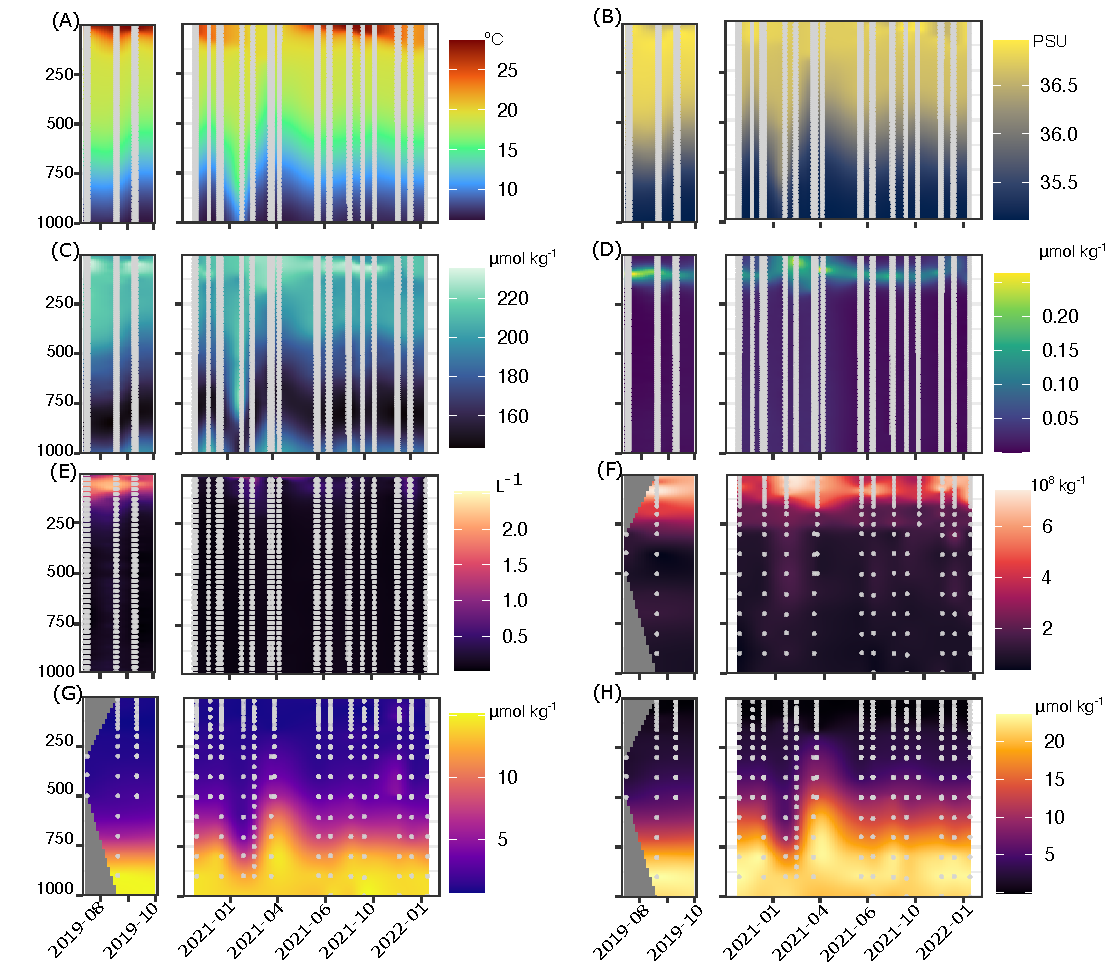
\includegraphics{images/02_environmental.pdf}

}

\caption{Environmental profiles across time-series of study period. Y
axis shows depth in meters. (A) Temperature. (B) Salinity. (C) Dissolved
Oxygen. (D) in situ chlorophyll fluorescence. (E) Particle concenctrion
(184 - 900\$\textbackslash mu m\$). (F) Bacteria Abundance. (G) Silica.
(H) Nitrate}

\end{figure}

Overall, particle concentration was high near the surface during the
2021 spring bloom, then moved deeper throughout the water column
attenuating throughout the lower epipelagic (Figure 2E). Similarly,
heterotrophic bacteria abundance was closely linked to overall
productivity, althrough there was a more consistent moderate-abundance
layer near the top of the mesopelagic (\textasciitilde250m) (Figure 2F).
Concurrent with the secondary fall production peak, there was also
higher particle concentration and bacterial abundance in the later
summer and early fall. Interestingly, while primary productivity
estimates from July-August were not that different between 2019 and 2021
(Figure 3A), chlorophyll-a florescence, particle concentration, and
bacterial abundance were much higher in 2019's summer/fall (Figure
2D-F). Inorganic nutrients (\(Si\) and \(NO_3\)) were generally well
stratified, with low concentrations in the epipelagic and increasing
throughout the mesopelagic. However, both nutrients did vary vertically
in accordance with the 2021 February downwelling and spring mixing
period (Figure 2G-H). Additionally, in the late fall of 2021, \(Si\)
concentrations were slightly elevated in the mid-mesopelagic (Figure
2G).

\begin{figure}

{\centering \includegraphics{images/03_prod-flux.pdf}

}

\caption{Primary productivity (A) and flux estimates from total mass
(B), carbon (C), and nitrogen (D). Values are from monthly cruises with
month displayed in corresponding colors. Absent data are shown by grey
bar.}

\end{figure}

Overall mass flux to the mesopelagic was highest during the 2021
February downwelling (Figure 3B). Generally, export was similarly high
during March, declining in April then increasing slightly throughout the
summer and early fall. While magnitude was slightly different, this
pattern was consistent with total mass, carbon and nitrogen fluxes
(Figure 3B-D). Higher mass, carbon and nitrogen flux also occurred in
the 2019 late summer - early fall period.

\hypertarget{rhizaria-abundance-and-distribution}{%
\subsubsection{Rhizaria abundance and
distribution}\label{rhizaria-abundance-and-distribution}}

Across all imaged mesozooplankton (\textgreater900\(\mu m\)), Rhizaria
comprised a considerable fraction of the total community. Considering
the total abundances of the observational period, Rhizaria comprised on
average, 42.6\% of all mesozooplankton abundance (Supplemental Figure
3). Copepods were the second most abundant, comprising 35.5\% and all
other living mesozooplankton were 22\%. The large contribution of
Rhizaria to the mesozooplankton community is most prominent in the
epipelagic, where they accounted for 47\% of all mesozooplankton
abundance. In the mesopelagic Rhizaria were a smaller fraction, at 38\%
in the upper layers (200-500m) and 37\% in the deeper mesopelagic
(500-1000m).

\begin{figure}

{\centering \includegraphics{images/04_vertical.pdf}

}

\caption{Average abundance of Rhizaria in 25m bins, across entire study
period. Shown are total Rhizaria (A), Acantharea (B), Collodaria (C),
Aulacanthidae (D), Foraminifera (E), Aulosphaeridae (F), Castanellidae
(G), Coelodendridae (H).}

\end{figure}

Average abundance of all Rhizaria had a bimodal distribution with
respect to depth. Total abundance was highest just below the surface
(0-100m), with secondary, wider peak occurring in the mid mesopelagic
(Figure 4A). Variation in depth binned abundance was large, likely due
to seasonal variability but also increased from the detection-risk
described in the methods. The vertical distribution pattern and
abundance varied considerably across taxonomic groups. Radiolaria were
some of the most abundant taxa observed, particularly in the epipelagic
(Figure 4, Figure 5A). Acantharea displayed a bimodal distribution
accounting for a large portion of the total Rhizaria pattern (Figure 4B,
Figure 5). The surface layers were largely comprised of Collodaria,
whose colonies were abundant (Figure 4C). The most abundant Phaeodaria,
Aulacanthidae, also had a bimodal pattern with the density was highest
in the lower mesopelagic (Figure 4D). Foraminifera had a similar bimodal
distribution, yet their overall average densities were much lower
(Figure 4E). Aulosphaeridae had low average density and was nearly
homogeneously distributed throughout the water column, although slightly
lower in the epipelagic (Figure 4F). Castanellidae were the only
Phaeodaria who appeared to be effectively restricted to the photic zone
(Figure 4G). Alternatively, Coelodendridae primarily occurred in the
lower mesopelagic (Figure 4H). A few individuals from the families
Tuscaroridae and Medusettidae were also observed in the mesopelagic, yet
they were much rarer (data not shown).

\begin{figure}

{\centering \includegraphics{images/05_seasonality.pdf}

}

\caption{Seasonality of Rhizaria integrated abundance for the epipelagic
(0-200m) (A), upper mesopelagic (200-500m) (B), lower mesopelagic
(500-1000m) (C). Data shown are the cruise mean integrated abundance in
the water column region colored for each taxon.}

\end{figure}

Between the monthly cruises, Rhizaria integrated abundance varied in the
epipelagic. Highest average abundance occurred in June 2021 and was
lowest during the winter months (Figure 5A). The 2019 later summer -
fall period also had much higher integrated abundance than similar
months in 2021. While the majority of integrated abundance in the
epipelagic was consistently attributable to Collodaria, Acanthrea
abundance occurred sporadically and could account for a large portion of
the total in some months (Figure 5A). The mesopelagic integrated
abundance was much more consistent across monthly cruises, although
average abundance was notably higher in 2019 (Figure 5B, 5C). The
community composition in the mesopelagic was more diverse, mostly
comprised of Phaeodaria families. However, Acantharea and unidentified
Rhizaria also were common members of the community (Figure 5B, C).

\hypertarget{body-size-throughout-the-water-column.}{%
\subsubsection{Body size throughout the water
column.}\label{body-size-throughout-the-water-column.}}

Very few taxa had consistent distributions throughout the water column.
Only Acanthrea, Foraminifera, Aulacanthidae, and Aulosphaeridae were
consistently abundant in the epipelagic and mesopelagic. To investigate
if the populations or morphologies shifted throughout the water column,
we compared the sizes (ESD) between mesopelagic and epipelagic groups
for each taxa. All groups were significantly different on average
(Wilcox Rank Sum p-value \textless0.001). Acantharea were smaller, on
average in the mesopelagic while all other taxa tended to be larger
(Figure 6).

\begin{figure}

{\centering \includegraphics{images/09_size-comp.pdf}

}

\caption{Comparison of average sizes (ESD) amongst Rhizaria taxa which
occurred throughout the water column.}

\end{figure}

\hypertarget{environmental-drivers-of-rhizaria-abundance}{%
\subsubsection{Environmental Drivers of Rhizaria
Abundance}\label{environmental-drivers-of-rhizaria-abundance}}

\begin{figure}

{\centering \includegraphics{images/06_tot-partials.pdf}

}

\caption{Partial effect plots from Generalized Additive Models (GAMs) of
all Rhizaria abundance. Models were constructed separately for depth
integrated abundance through the Epipelagic (0-200m) (A-G), Upper
Mesopelagic (200-500m) (H-J), and the Lower Mesopelagic (500-1000m)
(K-L). Each panel represents the partial effect of a GAM model term,
with smoothed relationship shown shaded with 95\% confidence intervals.
Individual points are depth integrated values for all Rhizaria from an
individual cast, colored by month.}

\end{figure}

For integrated abundance of all Rhizaria, the GAMs produced moderate
fits (\(R^2_{adj}\) = 0.406-0.603) (Table 1). In the epipelagic, there
were several significant predictor variables (Figure 7A-7G). This
included terms which are likely indicators of changing water masses;
Salinity (7E) and Temperature (7G). The model also had parameters
related to both heterotrophy (Particle concentration, 7A) and autotrophy
(Primary production, 7B). However the relationship to particle
concentration is weakly increasing trend while the primary productivity
effect appears to be influenced by a cruise with a high outlier for
increased primary productivity. The models for the mesopelagic regions
were much more reduced and the only significant effects were
particle-related terms (particle concentration and mass flux). In the
upper mesopelagic (Figure 7H-7J), final model included N flux, particle
concentration and a non-significant effect for Silica. The lower
mesopelagic (Figure 7K, 7L) only had model effects kept of total mass
flux and particle concentration. For both the upper and lower
mesopelagic, particle concentration had a clear, strong positive
relationship (Figure 7I, 7L).

\begin{longtable}[]{@{}
  >{\raggedright\arraybackslash}p{(\columnwidth - 8\tabcolsep) * \real{0.4300}}
  >{\raggedright\arraybackslash}p{(\columnwidth - 8\tabcolsep) * \real{0.3400}}
  >{\raggedright\arraybackslash}p{(\columnwidth - 8\tabcolsep) * \real{0.0800}}
  >{\raggedright\arraybackslash}p{(\columnwidth - 8\tabcolsep) * \real{0.0800}}
  >{\raggedright\arraybackslash}p{(\columnwidth - 8\tabcolsep) * \real{0.0800}}@{}}
\caption{Generalized Additive Model results for integrated total
Rhizaria abundance in different regions of the water column. edf =
estimated degrees of freedom, F = F-statistic, p = p-value. Models were
selected using a backwards-stepwise approach with a retention threshold
of p = 0.1 or a large enough reduction in model fit.}\tabularnewline
\toprule()
\begin{minipage}[b]{\linewidth}\raggedright
\textbf{Model}
\end{minipage} & \begin{minipage}[b]{\linewidth}\raggedright
Term
\end{minipage} & \begin{minipage}[b]{\linewidth}\raggedright
edf
\end{minipage} & \begin{minipage}[b]{\linewidth}\raggedright
F
\end{minipage} & \begin{minipage}[b]{\linewidth}\raggedright
p
\end{minipage} \\
\midrule()
\endfirsthead
\toprule()
\begin{minipage}[b]{\linewidth}\raggedright
\textbf{Model}
\end{minipage} & \begin{minipage}[b]{\linewidth}\raggedright
Term
\end{minipage} & \begin{minipage}[b]{\linewidth}\raggedright
edf
\end{minipage} & \begin{minipage}[b]{\linewidth}\raggedright
F
\end{minipage} & \begin{minipage}[b]{\linewidth}\raggedright
p
\end{minipage} \\
\midrule()
\endhead
\textbf{All Rhizaria Epipelagic} & Temperature & 0.7950 & 0.492 &
0.0440 \\
\(R^2_{adj}\)= 0.48 & Salinity & 2.4117 & 5.113 & \textless0.001 \\
& Silica & 2.1511 & 8.601 & \textless0.001 \\
& Bacteria Concentration & 0.8870 & 1.544 & \textless0.001 \\
& Avg Mass Flux & 1.4107 & 0.802 & 0.0211 \\
& Primary Productivity & 1.9280 & 2.736 & \textless0.001 \\
& Particle Concentration & 0.9151 & 2.136 & \textless0.001 \\
\textbf{All Rhizaria Upper Mesopelagic} & Silica & 0.6702 & 0.404 &
0.0814 \\
\(R^2_{adj}\)= 0.40 & Avg N Flux & 2.9524 & 3.172 & \textless0.001 \\
& Particle Concentration & 3.5568 & 11.82 & \textless0.001 \\
\textbf{All Rhizaria Lower Mesopelagic} & Avg Mass Flux & 2.036 & 2.953
& \textless0.001 \\
\(R^2_{adj}\)= 0.61 & Particle Concentration & 3.819 & 27.43 &
\textless0.001 \\
\bottomrule()
\end{longtable}

GAMs for individual taxa were much less consistent in their fits (Table
2). This is likely in part due to the high number of non-observations
for certain taxa. Note that due to low abundances, GAMs were not
constructed for Tuscaroridae or Medusettidae. Furthermore no,
significant terms were found for a model with Aulosphaeridae in the
epipelagic nor Foraminifera in the mesopelagic.

Epipelagic Acantharea were explained by several predictor variables and
had a good fit (\(R^2_{adj}\) = 0.539, Table 2, Supplemental FIgure 4).
Foraminifera had a good fitting GAM in the epipelagic (\(R^2_{adj}\) =
0.543). There were several significant explanatory variables, although
the clearest pattern was observed of high temperatures associated with
more Foraminifera abundance (Table 2, Supplemental Figure 4U).
Epipelagic Aulacanthidae similarly had several predictor variables which
were significant, including both water quality parameters and
particle/flux predictors (Table 2). There was a weak fit for Collodaria
in the epipelagic (\(R^2_{adj}\) = 0.16), although there was a
logit-like relationship where higher abundances tended to occur during
higher DO conditions in the surface waters (Supplemental Figure 4).
Castanellidae also had a weak model fit in the epipelagic (\(R^2_{adj}\)
= 0.228), although particle concentration was the strongest predictor
term (Table 2, Supplemental Figure 4).

\begin{longtable}[]{@{}
  >{\raggedright\arraybackslash}p{(\columnwidth - 8\tabcolsep) * \real{0.4300}}
  >{\raggedright\arraybackslash}p{(\columnwidth - 8\tabcolsep) * \real{0.3400}}
  >{\raggedright\arraybackslash}p{(\columnwidth - 8\tabcolsep) * \real{0.0800}}
  >{\raggedright\arraybackslash}p{(\columnwidth - 8\tabcolsep) * \real{0.0800}}
  >{\raggedright\arraybackslash}p{(\columnwidth - 8\tabcolsep) * \real{0.0800}}@{}}
\caption{Taxa-specific generalized additive models for different regions
of the water column.edf = estimated degrees of freedom, F = F-statistic,
p = p-value. Models were selected using a backwards-stepwise approach
with a retention threshold of p = 0.1 or a large enough reduction in
model fit.}\tabularnewline
\toprule()
\begin{minipage}[b]{\linewidth}\raggedright
Model
\end{minipage} & \begin{minipage}[b]{\linewidth}\raggedright
Term
\end{minipage} & \begin{minipage}[b]{\linewidth}\raggedright
edf
\end{minipage} & \begin{minipage}[b]{\linewidth}\raggedright
F
\end{minipage} & \begin{minipage}[b]{\linewidth}\raggedright
p
\end{minipage} \\
\midrule()
\endfirsthead
\toprule()
\begin{minipage}[b]{\linewidth}\raggedright
Model
\end{minipage} & \begin{minipage}[b]{\linewidth}\raggedright
Term
\end{minipage} & \begin{minipage}[b]{\linewidth}\raggedright
edf
\end{minipage} & \begin{minipage}[b]{\linewidth}\raggedright
F
\end{minipage} & \begin{minipage}[b]{\linewidth}\raggedright
p
\end{minipage} \\
\midrule()
\endhead
\textbf{Acantharea Epipelagic} & Temperature & 0.868 & 0.380 & 0.0935 \\
\(R^2_{adj}\)=0.539 & Salinity & 2.349 & 4.646 & \textless0.001 \\
& O2 & 2.501 & 5.493 & \textless0.001 \\
& Avg Mass Flux & 4.815 & 22.59 & \textless0.001 \\
& Bacteria & 1.608 & 1.360 & 0.00945 \\
& Particle Concentration & 0.877 & 1.414 & 0.00449 \\
\textbf{Acantharea Upper Mesopelagic} & Avg Mass Flux & 1.866 & 1.220 &
0.0166 \\
\(R^2_{adj}\)=0.197 & Avg N Flux & 2.208 & 3.100 & \textless0.001 \\
& Primary Productivity & 2.382 & 2.497 & \textless0.001 \\
& Particle Concentration & 0.724 & 0.521 & 0.0437 \\
\textbf{Acantharea Lower Mesopelagic} & Temperature & 1.958 & 2.986 &
\textless0.001 \\
\(R^2_{adj}\)=0.496 & Avg N Flux & 1.513 & 1.565 & 0.0037 \\
& Primary Productivity & 0.856 & 1.153 & 0.0045 \\
& Particle Concentration & 1.661 & 8.667 & \textless0.001 \\
\textbf{Aulacanthidae Epipelagic} & Temperature & 2.591 & 5.003 &
\textless0.001 \\
\(R^2_{adj}\)=0.394 & Salinity & 1.523 & 1.789 & 0.002 \\
& RFU & 0.872 & 1.315 & 0.0042 \\
& Bacteria & 0.808 & 0.833 & 0.0160 \\
& Primary Productivity & 2.622 & 9.160 & \textless0.001 \\
& Particle Concentration & 1.937 & 2.751 & \textless0.001 \\
\textbf{Aulacanthidae Upper Mesopelagic} & Avg C Flux & 1.675 & 1.408 &
0.0109 \\
\(R^2_{adj}\)=0.132 & Particle Concentration & 2.308 & 2.476 & 0.0013 \\
\textbf{Aulacanthidae Lower Mesopelagic} & Avg Mass Flux & 1.476 & 1.418
& 0.0076 \\
\(R^2_{adj}\)=0.308 & Particle Concentration & 2.457 & 7.756 &
\textless0.001 \\
\textbf{Aulosphaeridae Upper Mesopelagic} & Particle Concentration &
2.778 & 12.76 & \textless0.001 \\
\(R^2_{adj}\)=0.196 & & & & \\
\textbf{Aulosphaeridae Lower Mesopelagic} & Particle Concentration &
2.012 & 6.306 & \textless0.001 \\
\(R^2_{adj}\)=0.148 & & & & \\
\textbf{Castanellidae Epipelagic} & Salinity & 0.915 & 0.400 & 0.0935 \\
\(R^2_{adj}\)=0.228 & RFU & 0.912 & 2.052 & \textless0.001 \\
& Si & 2.018 & 3.656 & \textless0.001 \\
& Bacteria & 1.128 & 0.883 & 0.0170 \\
& Particle Concentration & 2.278 & 4.028 & \textless0.001 \\
\textbf{Coelodendridae Upper Mesopelagic} & Avg N Flux & 0.734 & 0.551 &
0.0527 \\
\(R^2_{adj}\)=0.09 & Particle Concentration & 0.965 & 5.102 &
\textless0.001 \\
\textbf{Coelodendridae Lower Mesopelagic} & Particle Concentration &
3.051 & 6.768 & \textless0.001 \\
\(R^2_{adj}\)=0.157 & & & & \\
\textbf{Collodaria Epipelagic} & Salinity & 0.926 & 2.267 &
\textless0.001 \\
\(R^2_{adj}\)=0.16 & O2 & 2.015 & 2.217 & \textless0.001 \\
& Bacteria & 1.843 & 2.100 & 0.0024 \\
\textbf{Foraminifera Epipelagic} & Temperature & 4.420 & 7.624 &
\textless0.001 \\
\(R^2_{adj}\)=0.543 & O2 & 0.799 & 0.788 & 0.023 \\
& Bacteria & 0.000 & 0.000 & 0.523 \\
& Avg N Flux & 1.847 & 3.022 & \textless0.001 \\
& Primary Productivity & 0.472 & 0.139 & 0.183 \\
& Particle Concentration & 1.685 & 2.955 & \textless0.001 \\
\bottomrule()
\end{longtable}

In the upper mesopelagic (200-500m), abundances were generally low
(Figure 4) so GAMs were only constructed for Acantharea, Aulacanthidae,
Aulosphaeridae, and Coelodendridae (Table 2). All these models had
generally poor fits (\(R^2_{adj}\) \textless{} 0.20). Yet, for all upper
mesopelagic models, particle concentration was a significant explanatory
variable (Table 2, Supplemental Figure 5). The lower mesopelagic also
had generally poor GAM fits for taxon specific models (\(R^2_{adj}\)
\textless0.31), with the exception of Acantharea (\(R^2_{adj}\) =
0.496). Acantharea in the lower mesopelagic was most clearly positively
associated with particle concentration (Supplemental Figure 6). For all
Phaeodaria with a significant model, particle concentration was a main
predictor variable (Table 2, Supplemental Figure 6).

\hypertarget{discussion}{%
\section{Discussion}\label{discussion}}

\hypertarget{overall-rhizaria-abundance-and-patterns}{%
\subsubsection{Overall Rhizaria abundance and
patterns}\label{overall-rhizaria-abundance-and-patterns}}

In the epipelagic Rhizaria exhibited a notable seasonal pattern.
Rhizaria abundances were higher in the summer months and lower during
the winter. During a prior time period, Blanco-Bercial \emph{et al.}
(2022) noted that there is considerable seasonality in the community
composition of all protists. Despite the seasonality of Rhizaria
abundance, community composition was relatively consistent, with
Collodaria representing the bulk of the community. It should be noted
that the overall taxonomic resolution of the UVP5 is fairly low, so
there may be a switching of species within the broad groups identified
in this study which were not captured. Throughout the mesopelagic,
month-to-month variation in 2021 was relatively low. Again, this is
consistent with observations from metabarcoding of the whole protist
community in the same study region (Blanco-Bercial \emph{et al.}, 2022).
This finding is not surprising as the overall seasonal variation in
environmental conditions in this region were low.

Overall Rhizaria were the most commonly identified group of mesoplankton
throughout the study period. We do note that the UVP5 commonly captures
\emph{Trichodesmium} colonies, yet these were excluded in this
comparison as they are strictly autotrophs. It should be noted that
previous work has suggested that avoidance behavior with the UVP is
possible, at times likely, for visual and highly mobile zooplankton
(Barth and Stone, 2022). Thus, the percent contribution reported here
(42.7\%) of Rhizaria to the total mesozooplankton community may be
inflated due to under sampling of organisms such as Euphausiids and
Chaetognaths which have quick escape responses. Regardless, it is worth
noting that in the same region, with data collected in 2012 and 2013
using similar calculation methods, Biard \emph{et al.} (2016) estimated
large Rhizaria only contribute 15\% of the total mesozooplankton
community in the upper 500m. Likely, Rhizaria display considerable
interannual variability. In the present study, we noticed considerably
higher Rhizaria abundance throughout the water column in 2019 compared
to 2021. Similarly, in the California Current a multi-year study of
Aulosphaeridae saw considerable variation between years (Biard \emph{et
al.}, 2018). To truly understand the drivers of interannual variability
however, sustained observations of Rhizaria over longer time periods are
required.

\hypertarget{relationship-to-environmental-parameters}{%
\subsubsection{Relationship to environmental
parameters}\label{relationship-to-environmental-parameters}}

In general, the fit of most GAMs were moderate to poor. One possible
reason for the poor fits may have been that for some taxa, conditions
were not variable enough to capture a range of conditions at which they
may exist. For instance, Collodaria were the most abundant taxa
observed, yet the fit of their GAM was particularly poor. In studies
which covered a wider range of parameters, Collodaria has been shown to
strongly vary with changes in parameters such as temperature,
chlorophyll-a, mixing, and water clarity (Biard \emph{et al.}, 2017;
Biard and Ohman, 2020). Alternatively, Acantharea had relatively good
fitting GAMs. These taxa also had some of the largest variation from
month to month on cruises. Thus, it may be that in the oligotrophic, the
relatively stable conditions can support certain taxa while others are
more sporadic. It should also be noted that due to the challenge of
adequately sampling enough volume to overcome low-detection issues, GAMs
were run on integrated data. However, variation with environmental
parameters throughout the water column are likely, just not captured in
the modelling aspect of this study. Future studies which are able to
account for detection biases in finer vertical resolution of Rhizaria
may improve ecological models of their abundance. One consistent
parameter which had significant positive associations was particle
concentration. This observation is not surprising as most Rhizaria
likely to some extent engage in flux feeding.

\hypertarget{vertical-structure-and-trophic-roles}{%
\subsubsection{Vertical Structure and Trophic
Roles}\label{vertical-structure-and-trophic-roles}}

In this study we present a clear pattern of vertical zonation between
different Rhizaria groups. Largely, the taxonomic composition and
vertical positioning were similar to Rhizaria zonation in the California
Current Ecosystem (Biard and Ohman, 2020). It should be noted however,
that the secondary abundance peak reported in the present study is lower
in magnitude. This is likely due to the more oligotrophic nature of the
study region, were the euphotic zone penetrates deeper into the water
column. Most prevalent in the epipelagic were Collodaria. These
mixotrophic Radiolaria have long been reported to contribute to primary
productivity in the euphotic zone (Michaels \emph{et al.}, 1995; Dennett
\emph{et al.}, 2002). Collodaria are thought to be particularly
successful globally in oligotrophic regions due to their photosymbiotic
relationships (Biard \emph{et al.}, 2016, 2017). We observed the highest
abundance of Collodaria during June 2021, supporting the notion they can
thrive during the typically low-nutrient conditions of summer
stratification. However, Collodaria also increased during the spring
mixing period, suggesting that they can thrive during conditions which
may typically be thought to favor autotrophs. Furthermore, while
Collodaria were primarily absent from below 250m, there were a few
instances of deeper colonies being observed. Global investigations of
polycystine flux, suggest that deep-Collodaria in oligotrophic regions
may be a consequence of isothermal submersion (Boltovskoy, 2017).
Alternatively, surface waters at BATS often mix into the mode water
during the seasonal mixing, so Collodaria in the deeper waters may be a
result of diapyncal mixing. Another effectively exclusively epipelagic
Rhizaria was the Phaeodaria family of Castanellidae. All Phaeodaria are
thought to be fully heterotrophic (Nakamura and Suzuki, 2015),
nonetheless a number of studies, including this one, report
Castanellidae to be typically found in the lower epipelagic (Zasko and
Rusanov, 2005; Biard \emph{et al.}, 2018; Biard and Ohman, 2020). It
should be considered that perhaps Castanellidae specializes in feeding
on sinking particles directly at the base of the epipelagic. Given it's
smaller size (Nakamura and Suzuki, 2015), Castanellidae does not need a
large diameter to efficiently flux feed at the typically particle rich
region of the lower epipelagic.

The mesopelagic generally was home to known heterotrophic organisms,
particularly for those which were constrained to exclusively occupy
deeper waters. This is consistent with Blanco-Bercial \emph{et al.}
(2022)'s observation of an auto-/mixotroph to heterotroph gradient in
local protist community as well as global patterns in Rhizaria ecology
(Laget \emph{et al.}, 2024). The upper mesopelagic interestingly had
relatively low total abundance. This low-abundance region likely
reflects the dynamics of productivity and export throughout the water
column. While productivity and thus sinking particles for flux feeders
are high in the euphotic zone, much of this is attenuated throughout the
epipelagic. So, while the base of the epipelagic may provide a rich
feeding environment for Castanellidae, smaller protists, or
heterotrophic bacteria (Figure 2F), the region from 200-500m might be
otherwise food poor. Perhaps it is more advantageous for Rhizaria to
situate deeper, in darker regions of the twilight zone where visual
predators and vertically migrating organisms may not feed on them. Also
it should be noted that Phaeodaria utilize silica to build their opaline
tests, and silica concentrations started to increase around 500m (Figure
2G). However, \(Si\) was not a significant term for any taxon-specific
model in the mesopelagic. Aulosphaeridae was only found to have
significant relationships, although weak fits, to particle concentration
in the mesopelagic. In our study, while consistently observed, overall
abundances of Aulosphaeridae were very low. In the Pacific Ocean, on
California's Coast, much higher abundances of Aulosphaeridae have been
reported (Zasko and Rusanov, 2005; Biard and Ohman, 2020) and they have
massive potential to impact silica export (Biard \emph{et al.}, 2018).
Coelodendridae were also seemingly restricted to the deeper section of
the mesopelagic. This is interesting given that in the California
Current, (Biard and Ohman, 2020) found a bimodal distribution in
Coelodendridae. There are several morphotypes corresponding to different
taxa of Coelodendridae (Nakamura and Suzuki, 2015; Biard and Ohman,
2020). So it may be that only a few types of Coelodendridae were
observed in this study, while the epipelagic variety was not.
Alternatively, the lower epipelagic of the extremely productive
California Current may provide adequate habitat for Coelodendridae,
which is not available in the oligotrophic Sargasso Sea.

A number of taxa were found to have a bimodal distribution, with sizable
populations in both the epipelagic and mesopelagic. Aulacanthidae had a
bimodal distribution, although abundances were highest in the lower
mesopelagic. Foraminifera also had a bimodal distribution. Some lineages
of Foraminifera are known to host photosymbionts (Kimoto, 2015; Biard,
2022b), however they are also efficient predators commonly seen
throughout the mesopelagic (Caron and Be, 1984; Gaskell \emph{et al.},
2019). Thus it is not surprising to find their presence in both
locations of the water column. Foraminifera are also known to vary their
vertical distribution across their life cycle in phase with lunar cycles
(Bijma \emph{et al.}, 1990; Kimoto, 2015; Gaskell \emph{et al.}, 2019;
Biard, 2022b). However, the sampling scheme of the BATS program does not
capture this frequency and was not investigated in the present study.

Acantharea also had a bimodal distribution, with much more sizable
abundances than Aulacanthidae or Foraminifera. Most prior studies of
Acantharea vertical distribution found them concentrated in near surface
layers of the water column Zasko and Rusanov (2005). This would support
the paradigm that large Acantharea abundances may be supported by their
mixotrophic abilities (Michaels \emph{et al.}, 1995; Suzuki and Not,
2015). While the UVP5 images cannot distinguish between mixotrophic and
heterotrophic Acantharea, the GAMs constructed for Acantharea abundance
found positive associations with particle concentration and mass flux,
suggesting a higher reliance on heterotrophy. Recently Mars Brisbin
\emph{et al.} (2020) described apparent predator behavior amongst
near-surface Acantharea. Thus it is likely that epipelagic Acantharea
may commonly be heterotrophic or mixotrophic with an increased reliance
on heterotrophy. Yet, it should be noted in the Sargasso Sea, both
heterotrophic and symbiotic lineages of Acantharea have been reported
(Blanco-Bercial \emph{et al.}, 2022). Additionally, Michaels (1988)
noted that the majority of Acantharea (by abundance) were smaller than
160\(\mu m\). While that estimate may be inflated due to inability to
capture larger cells, small Acantharea were not captured in the present
study. Thus, trophic strategy may shift based on sizes of Acantharea.

Decelle \emph{et al.} (2013) proposed a hypothetical life cycle for
cyst-bearing (strictly heterotrophic) Acantharea. This hypothesized life
cycle suggests that epipelagic Acantharea are adult populations, which
form cysts that sink into the mesopelagic, then reproduce and rise.
Furthermore, given that horizontal transfer of symbionts between
generations of Acantharea is unlikely due to their spawning behavior,
the newly spawned mesopelagic Acantharea are not necessarily required to
rapidly return to the photic zone (Decelle \emph{et al.}, 2012, 2013).
This hypothesis predicts that Acantharea in the mesopelagic would be
smaller (Decelle \emph{et al.}, 2013). Mars Brisbin \emph{et al.} (2020)
provided some support for this hypothesis, with a significant decrease
in Acantharea sizes with depth. Although the authors also observed low
abundances in the mesopelagic and noted that the smaller sizes may be
due to lower food availability (Mars Brisbin \emph{et al.}, 2020). Since
food is more scarce in the mesopelagic, nutritional quality lower (Kim
\emph{et al.}, 2018), yet flux feeders would likely grow larger to
increase their feeding range (Stukel \emph{et al.}, 2018; Biard and
Ohman, 2020). In the data collecting in this study, Acantharea in the
mesopelagic were significantly smaller than the epipelagic, despite the
other bimodal taxa (Foraminifera and Aulacanthidae) being significantly
larger with depth. This provides added support for the hypothesis that
cyst-forming Acantharea may utilize different sections of the water
column throughout their life cycle. However to further investigate this,
more work is needed with higher temporal and taxonomic resolution.

\hypertarget{conclusions-and-considerations}{%
\subsubsection{Conclusions and
Considerations}\label{conclusions-and-considerations}}

This study provides a detailed look at Rhizaria abundance over time
throughout the water column in a major oligotrophic gyre. We show that
their abundances are generally related to particle concentration and
flux, although lack of environmental variability may have reduced the
fit of our GAMs. Considering the potential role of Rhizaria in the
biological carbon pump, they may have a somewhat mixed role. In the
shallower regions, they may be an attenuating force on sinking particles
(Stukel \emph{et al.}, 2019). However, once consumed and repackaged by
larger Rhizaria, they can sink quicker and contribute more to overall
flux (Michaels, 1988). Thus, Rhizaria may act as an aggregation
mechanism. However, to truly test this, more work is needed measuring
Rhizaria flux.

The vertical partitioning documented in this study do support the
hypothesis that mixotrophic rhizaria will occupy shallower waters while
deeper waters are dominated by heterotrophy. However the degree to which
mixotrophic Rhizaria in the euphotic zone rely on heterotrophy versus
symbiosis is uncertain. Collodaria were recorded as consistent and
dominant members of the near surface region. These organisms have the
potential to contribute considerably to the otherwise low productivity
of oligotrophic regions. However, their role in food webs is not well
understood. While this study represents a step forward in our
understanding of Rhizaria, further research is needed to better
characterize their ecology and role in biogeochemical cycling. To fully
understand the functioning of the oceans, not only carbon or nitrogen,
but other elements such as silica or strontium, extended work addressing
the interannual patterns in Rhizaria, their biotic interactions, and the
key biological rates that impact ocean biogeochemistry, will be
required.

\hypertarget{references}{%
\section{References:}\label{references}}

\hypertarget{refs}{}
\begin{CSLReferences}{1}{0}
\leavevmode\vadjust pre{\hypertarget{ref-anderson2014}{}}%
Anderson, O. R. (2014)
\href{https://doi.org/10.4467/16890027AP.13.0019.1116}{Living Together
in the Plankton: A Survey of Marine Protist Symbioses}. \emph{Acta
Protozoologica}, \textbf{53}, 29--38.

\leavevmode\vadjust pre{\hypertarget{ref-anderson1976}{}}%
Anderson, O. R. and Bé, A. W. H. (1976)
\href{https://doi.org/10.2307/1540498}{A CYTOCHEMICAL FINE STRUCTURE
STUDY OF PHAGOTROPHY IN A PLANKTONIC FORAMINIFER, {\emph{HASTIGERINA
PELAGICA}} (d'ORBIGNY)}. \emph{The Biological Bulletin}, \textbf{151},
437--449.

\leavevmode\vadjust pre{\hypertarget{ref-barth2022}{}}%
Barth, A. and Stone, J. (2022)
\href{https://www.frontiersin.org/articles/10.3389/fmars.2022.898057}{Comparison
of an in situ imaging device and net-based method to study
mesozooplankton communities in an oligotrophic system}. \emph{Frontiers
in Marine Science}, \textbf{9}.

\leavevmode\vadjust pre{\hypertarget{ref-barth2024}{}}%
Barth, A. and Stone, J. (2024)
\href{https://doi.org/10.1093/plankt/fbae023}{Understanding the picture:
The promis and challenges of in-situ imagery data in the study of
plankton ecology}. \emph{Journal of Plankton Research: Horizons}, 1--15.

\leavevmode\vadjust pre{\hypertarget{ref-benfield1996}{}}%
Benfield, M. C., Davis, C. S., Wiebe, P. H., Gallager, S. M., Gregory
Lough, R., and Copley, N. J. (1996)
\href{https://doi.org/10.1016/S0967-0645(96)00044-6}{Video Plankton
Recorder estimates of copepod, pteropod and larvacean distributions from
a stratified region of Georges Bank with comparative measurements from a
MOCNESS sampler}. \emph{Deep Sea Research Part II: Topical Studies in
Oceanography}, \textbf{43}, 1925--1945.

\leavevmode\vadjust pre{\hypertarget{ref-biard2022b}{}}%
Biard, T. (2022a)
\href{https://doi.org/10.1111/1462-2920.16004}{Diversity and ecology of
Radiolaria in modern oceans}. \emph{Environmental Microbiology},
\textbf{24}, 2179--2200.

\leavevmode\vadjust pre{\hypertarget{ref-biard2022}{}}%
Biard, T. (2022b)
\href{https://doi.org/10.1002/9780470015902.a0029469}{Rhizaria}.
Encyclopeida of Life Sciences, pp. 1--11.

\leavevmode\vadjust pre{\hypertarget{ref-biard2017}{}}%
Biard, T., Bigeard, E., Audic, S., Poulain, J., Gutierrez-Rodriguez, A.,
Pesant, S., Stemmann, L., and Not, F. (2017)
\href{https://doi.org/10.1038/ismej.2017.12}{Biogeography and diversity
of Collodaria (Radiolaria) in the global ocean}. \emph{The ISME
Journal}, \textbf{11}, 1331--1344.

\leavevmode\vadjust pre{\hypertarget{ref-biard2018}{}}%
Biard, T., Krause, J. W., Stukel, M. R., and Ohman, M. D. (2018)
\href{https://doi.org/10.1029/2018GB005877}{The Significance of Giant
Phaeodarians (Rhizaria) to Biogenic Silica Export in the California
Current Ecosystem}. \emph{Global Biogeochemical Cycles}, \textbf{32},
987--1004.

\leavevmode\vadjust pre{\hypertarget{ref-biard2020}{}}%
Biard, T. and Ohman, M. D. (2020)
\href{https://doi.org/10.1002/lno.11472}{Vertical niche definition of
test-bearing protists (Rhizaria) into the twilight zone revealed by in
situ imaging}. \emph{Limnology and Oceanography}, \textbf{65},
2583--2602.

\leavevmode\vadjust pre{\hypertarget{ref-biard2016}{}}%
Biard, T., Stemmann, L., Picheral, M., Mayot, N., Vandromme, P., Hauss,
H., Gorsky, G., Guidi, L., \emph{et al.} (2016)
\href{https://doi.org/10.1038/nature17652}{In situ imaging reveals the
biomass of giant protists in the global ocean}. \emph{Nature},
\textbf{532}, 504--507.

\leavevmode\vadjust pre{\hypertarget{ref-bijma1990}{}}%
Bijma, J., Erez, J., and Hemleben, C. (1990)
\href{https://epic.awi.de/id/eprint/6096/1/Bij1990a.pdf}{Lunar and
semi-luan reproductive cycles in some spinose planktonic foraminifers}.
\emph{Journal of Foraminiferal Research}, \textbf{20}, 117--127.

\leavevmode\vadjust pre{\hypertarget{ref-blanco-bercial2020}{}}%
Blanco-Bercial, L. (2020)
\href{https://www.frontiersin.org/articles/10.3389/fmars.2020.00173}{Metabarcoding
analyses and seasonality of the zooplankton community at BATS}.
\emph{Frontiers in Marine Science}, \textbf{7}.

\leavevmode\vadjust pre{\hypertarget{ref-blanco-bercial2022}{}}%
Blanco-Bercial, L., Parsons, R., Bolaños, L. M., Johnson, R.,
Giovannoni, S. J., and Curry, R. (2022)
\href{https://www.frontiersin.org/articles/10.3389/fmars.2022.897140}{The
protist community traces seasonality and mesoscale hydrographic features
in the oligotrophic sargasso sea}. \emph{Frontiers in Marine Science},
\textbf{9}.

\leavevmode\vadjust pre{\hypertarget{ref-boltovskoy2017}{}}%
Boltovskoy, D. (2017)
\href{https://doi.org/10.1093/plankt/fbx003}{Vertical distribution
patterns of radiolaria polycystina (protista) in the world ocean: Living
ranges, isothermal submersion and settling shells}. \emph{Journal of
Plankton Research}, \textbf{39}, 330--349.

\leavevmode\vadjust pre{\hypertarget{ref-boltovskoy1993}{}}%
Boltovskoy, D., Alder, V. A., and Abelmann, A. (1993)
\href{https://doi.org/10.1016/0967-0637(93)90036-3}{Annual flux of
radiolaria and other shelled plankters in the eastern equatorial
atlantic at 853 m: seasonal variations and polycystine species-specific
responses}. \emph{Deep Sea Research Part I: Oceanographic Research
Papers}, \textbf{40}, 1863--1895.

\leavevmode\vadjust pre{\hypertarget{ref-caron2016}{}}%
Caron, D. A. (2016)
\href{https://www.nature.com/articles/nature17892}{The rise of rhizaria
\textbar{} nature}. \emph{Nature}, \textbf{532}, 444--445.

\leavevmode\vadjust pre{\hypertarget{ref-caron1984}{}}%
Caron, D. A. and Be, A. W. H. (1984) PREDICTED AND OBSERVED FEEDING
RATES OF THE SPINOSE PLANKTONIC FORAMINIFER. \emph{BULLETIN OF MARINE
SCIENCE}, \textbf{35}.

\leavevmode\vadjust pre{\hypertarget{ref-caron1995}{}}%
Caron, D. A., Michaels, A. F., Swanberg, N. R., and Howse, F. A. (1995)
\href{https://doi.org/10.1093/plankt/17.1.103}{Primary productivity by
symbiont-bearing planktonic sarcodines (acantharia, radiolaria,
foraminifera) in surface waters near bermuda}. \emph{Journal of Plankton
Research}, \textbf{17}, 103--129.

\leavevmode\vadjust pre{\hypertarget{ref-cohen2023}{}}%
Cohen, N. R., Krinos, A. I., Kell, R. M., Chmiel, R. J., Moran, D. M.,
McIlvin, M. R., Lopez, P. Z., Barth, A., \emph{et al.} (2023)
\href{https://doi.org/10.1101/2023.11.20.567900}{Microeukaryote
metabolism across the western North Atlantic Ocean revealed through
autonomous underwater profiling}.

\leavevmode\vadjust pre{\hypertarget{ref-decelle2015}{}}%
Decelle, J., Colin, S., and Foster, R. A. (2015)
\href{https://doi.org/10.1007/978-4-431-55130-0_19}{Photosymbiosis in
Marine Planktonic Protists}. In Ohtsuka, S., Suzaki, T., Horiguchi, T.,
Suzuki, N., and Not, F. (eds). Springer Japan, Tokyo, pp. 465--500.

\leavevmode\vadjust pre{\hypertarget{ref-decelle2013}{}}%
Decelle, J., Martin, P., Paborstava, K., Pond, D. W., Tarling, G., Mahé,
F., De Vargas, C., Lampitt, R., \emph{et al.} (2013)
\href{https://doi.org/10.1371/journal.pone.0053598}{Diversity, Ecology
and Biogeochemistry of Cyst-Forming Acantharia (Radiolaria) in the
Oceans}. \emph{PLoS ONE}, \textbf{8}, e53598.

\leavevmode\vadjust pre{\hypertarget{ref-decelle2012}{}}%
Decelle, J., Siano, R., Probert, I., Poirier, C., and Not, F. (2012)
\href{https://doi.org/10.1007/s13199-012-0195-x}{Multiple microalgal
partners in symbiosis with the acantharian Acanthochiasma sp.
(Radiolaria)}. \emph{Symbiosis}, \textbf{58}, 233--244.

\leavevmode\vadjust pre{\hypertarget{ref-dennett2002}{}}%
Dennett, M. R., Caron, D. A., Michaels, A. F., Gallager, S. M., and
Davis, C. S. (2002) \href{https://doi.org/10.1093/plankt/24.8.797}{Video
plankton recorder reveals high abundances of colonial radiolaria in
surface waters of the central north pacific}. \emph{Journal of Plankton
Research}, \textbf{24}, 797--805.

\leavevmode\vadjust pre{\hypertarget{ref-drago2022}{}}%
Drago, L., Panaïotis, T., Irisson, J.-O., Babin, M., Biard, T.,
Carlotti, F., Coppola, L., Guidi, L., \emph{et al.} (2022)
\href{https://doi.org/10.3389/fmars.2022.894372}{Global Distribution of
Zooplankton Biomass Estimated by In Situ Imaging and Machine Learning}.
\emph{Frontiers in Marine Science}, \textbf{9}.

\leavevmode\vadjust pre{\hypertarget{ref-gaskell2019}{}}%
Gaskell, D. E., Ohman, M. D., and Hull, P. M. (2019)
\href{https://doi.org/10.2113/gsjfr.49.4.390}{Zooglider-based
measurements of planktonic foraminifera in the california current
system}. \emph{Journal of Foraminiferal Research}, \textbf{49},
390--404.

\leavevmode\vadjust pre{\hypertarget{ref-gorsky2010}{}}%
Gorsky, G., Ohman, M. D., Picheral, M., Gasparini, S., Stemmann, L.,
Romagnan, J.-B., Cawood, A., Pesant, S., \emph{et al.} (2010)
\href{https://doi.org/10.1093/plankt/fbp124}{Digital zooplankton image
analysis using the ZooScan integrated system}. \emph{Journal of Plankton
Research}, \textbf{32}, 285--303.

\leavevmode\vadjust pre{\hypertarget{ref-gowing1989}{}}%
Gowing, M. M. (1989) \href{https://doi.org/10.1007/BF00391069}{Abundance
and feeding ecology of Antarctic phaeodarian radiolarians}. \emph{Marine
Biology}, \textbf{103}, 107--118.

\leavevmode\vadjust pre{\hypertarget{ref-gutierrez-rodriguez2019}{}}%
Gutierrez-Rodriguez, A., Stukel, M. R., Lopes dos Santos, A., Biard, T.,
Scharek, R., Vaulot, D., Landry, M. R., and Not, F. (2019)
\href{https://doi.org/10.1038/s41396-018-0322-7}{High contribution of
Rhizaria (Radiolaria) to vertical export in the California Current
Ecosystem revealed by DNA metabarcoding}. \emph{The ISME Journal},
\textbf{13}, 964--976.

\leavevmode\vadjust pre{\hypertarget{ref-gutiuxe9rrez-rodruxedguez2022}{}}%
Gutiérrez-Rodríguez, A., Lopes dos Santos, A., Safi, K., Probert, I.,
Not, F., Fernández, D., Gourvil, P., Bilewitch, J., \emph{et al.} (2022)
\href{https://doi.org/10.1016/j.pocean.2022.102809}{Planktonic protist
diversity across contrasting subtropical and subantarctic waters of the
southwest pacific}. \emph{Progress in Oceanography}, \textbf{206},
102809.

\leavevmode\vadjust pre{\hypertarget{ref-haekel1887}{}}%
Haekel, E. (1887)
\emph{\href{https://www.gutenberg.org/cache/epub/44527/pg44527-images.html}{Report
on the radiolaria collected by h.m.s. Challenger during the years
1873-1876, plates, by ernst haeckel}}.

\leavevmode\vadjust pre{\hypertarget{ref-hull2011}{}}%
Hull, P. M., Osborn, K. J., Norris, R. D., and Robison, B. H. (2011)
\href{https://doi.org/10.4319/lo.2011.56.2.0562}{Seasonality and depth
distribution of a mesopelagic foraminifer, Hastigerinella digitata, in
Monterey Bay, California}. \emph{Limnology and Oceanography},
\textbf{56}, 562--576.

\leavevmode\vadjust pre{\hypertarget{ref-ikenoue2019}{}}%
Ikenoue, T., Kimoto, K., Okazaki, Y., Sato, M., Honda, M. C., Takahashi,
K., Harada, N., and Fujiki, T. (2019)
\href{https://doi.org/10.1029/2019GB006258}{Phaeodaria: An Important
Carrier of Particulate Organic Carbon in the Mesopelagic Twilight Zone
of the North Pacific Ocean}. \emph{Global Biogeochemical Cycles},
\textbf{33}, 1146--1160.

\leavevmode\vadjust pre{\hypertarget{ref-kim2018}{}}%
Kim, B. K., Lee, S., Ha, S.-Y., Jung, J., Kim, T. W., Yang, E. J., Jo,
N., Lim, Y. J., \emph{et al.} (2018)
\href{https://doi.org/10.1002/2017JC013457}{Vertical Distributions of
Macromolecular Composition of Particulate Organic Matter in the Water
Column of the Amundsen Sea Polynya During the Summer in 2014}.
\emph{Journal of Geophysical Research: Oceans}, \textbf{123},
1393--1405.

\leavevmode\vadjust pre{\hypertarget{ref-kimoto2015}{}}%
Kimoto, K. (2015)
\href{https://doi.org/10.1007/978-4-431-55130-0_7}{Planktic
foraminifera}. pp. 129--178.

\leavevmode\vadjust pre{\hypertarget{ref-knap1997}{}}%
Knap, A. H., Michaels, A. F., Steinberg, D. K., Bahr, F., Bates, N. R.,
Bell, S., Countway, P., Close, A. R., \emph{et al.} (1997)
\href{https://eprints.soton.ac.uk/361194/}{BATS methods manual, version
4}.

\leavevmode\vadjust pre{\hypertarget{ref-laget2024}{}}%
Laget, M., Drago, L., Panaïotis, T., Kiko, R., Stemmann, L., Rogge, A.,
Llopis-Monferrer, N., Leynaert, A., \emph{et al.} (2024)
\href{https://doi.org/10.1038/s41467-024-47651-4}{Global census of the
significance of giant mesopelagic protists to the marine carbon and
silicon cycles}. \emph{Nature Communications}, \textbf{15}, 3341.

\leavevmode\vadjust pre{\hypertarget{ref-lee2006}{}}%
Lee, J. J. (2006)
\href{https://dalspace.library.dal.ca/bitstream/handle/10222/78255/VOLUME\%2042-NUMBER\%202-2006-PAGE\%2063.pdf?sequence=1}{Algal
symbiosis in larger foraminifera}. \emph{Symbiosis}, \textbf{42},
63--75.

\leavevmode\vadjust pre{\hypertarget{ref-llopismonferrer2022}{}}%
Llopis Monferrer, N., Biard, T., Sandin, M. M., Lombard, F., Picheral,
M., Elineau, A., Guidi, L., Leynaert, A., \emph{et al.} (2022)
\href{https://www.frontiersin.org/articles/10.3389/fmars.2022.895995}{Siliceous
rhizaria abundances and diversity in the mediterranean sea assessed by
combined imaging and metabarcoding approaches}. \emph{Frontiers in
Marine Science}, \textbf{9}.

\leavevmode\vadjust pre{\hypertarget{ref-lomas2013}{}}%
Lomas, M. W., Bates, N. R., Johnson, R. J., Knap, A. H., Steinberg, D.
K., and Carlson, C. A. (2013)
\href{https://doi.org/10.1016/j.dsr2.2013.01.008}{Two decades and
counting: 24-years of sustained open ocean biogeochemical measurements
in the Sargasso Sea}. \emph{Deep Sea Research Part II: Topical Studies
in Oceanography}, \textbf{93}, 16--32.

\leavevmode\vadjust pre{\hypertarget{ref-lombard2019}{}}%
Lombard, F., Boss, E., Waite, A. M., Vogt, M., Uitz, J., Stemmann, L.,
Sosik, H. M., Schulz, J., \emph{et al.} (2019)
\href{https://www.frontiersin.org/articles/10.3389/fmars.2019.00196}{Globally
consistent quantitative observations of planktonic ecosystems}.
\emph{Frontiers in Marine Science}, \textbf{6}.

\leavevmode\vadjust pre{\hypertarget{ref-marra2011}{}}%
Marra, G. and Wood, S. N. (2011)
\href{https://doi.org/10.1016/j.csda.2011.02.004}{Practical variable
selection for generalized additive models}. \emph{Computational
Statistics \& Data Analysis}, \textbf{55}, 2372--2387.

\leavevmode\vadjust pre{\hypertarget{ref-marsbrisbin2020}{}}%
Mars Brisbin, M., Brunner, O. D., Grossmann, M. M., and Mitarai, S.
(2020) \href{https://doi.org/10.1002/lno.11567}{Paired high-throughput,
in situ imaging and high-throughput sequencing illuminate acantharian
abundance and vertical distribution}. \emph{Limnology and Oceanography},
\textbf{65}, 2953--2965.

\leavevmode\vadjust pre{\hypertarget{ref-mcgillicuddy1998}{}}%
McGillicuddy, D. J., Robinson, A. R., Siegel, D. A., Jannasch, H. W.,
Johnson, R., Dickey, T. D., McNeil, J., Michaels, A. F., \emph{et al.}
(1998) \href{https://doi.org/10.1038/28367}{Influence of mesoscale
eddies on new production in the Sargasso Sea}. \emph{Nature},
\textbf{394}, 263--266.

\leavevmode\vadjust pre{\hypertarget{ref-michaels1988}{}}%
Michaels, A. F. (1988)
\href{https://doi.org/10.1007/BF00391052}{Vertical distribution and
abundance of Acantharia and their symbionts}. \emph{Marine Biology},
\textbf{97}, 559--569.

\leavevmode\vadjust pre{\hypertarget{ref-michaels1995}{}}%
Michaels, A. F., Caron, D. A., Swanberg, N. R., Howse, F. A., and
Michaels, C. M. (1995)
\href{https://doi.org/10.1093/plankt/17.1.131}{Planktonic sarcodines
(Acantharia, Radiolaria, Foraminifera) in surface waters near Bermuda:
abundance, biomass and vertical flux}. \emph{Journal of Plankton
Research}, \textbf{17}, 131--163.

\leavevmode\vadjust pre{\hypertarget{ref-michaels1996}{}}%
Michaels, A. F. and Knap, A. H. (1996)
\href{https://doi.org/10.1016/0967-0645(96)00004-5}{Overview of the U.S.
JGOFS Bermuda Atlantic Time-series Study and the Hydrostation S
program}. \emph{Deep Sea Research Part II: Topical Studies in
Oceanography}, \textbf{43}, 157--198.

\leavevmode\vadjust pre{\hypertarget{ref-nakamura2023}{}}%
Nakamura, Y., Itagaki, H., Tuji, A., Shimode, S., Yamaguchi, A., Hidaka,
K., and Ogiso-Tanaka, E. (2023)
\href{https://doi.org/10.1111/1462-2920.16524}{DNA metabarcoding focused
on difficult-to-culture protists: An effective approach to clarify
biological interactions}. \emph{Environmental Microbiology},
\textbf{25}, 3630--3638.

\leavevmode\vadjust pre{\hypertarget{ref-nakamura2015}{}}%
Nakamura, Y. and Suzuki, N. (2015)
\href{https://link.springer.com/chapter/10.1007/978-4-431-55130-0_9}{Phaeodaria:
Diverse marine cercozoans of world-wide distribution}. Springer, pp.
223--249.

\leavevmode\vadjust pre{\hypertarget{ref-ohman2019a}{}}%
Ohman, M. D. (2019) \href{https://doi.org/10.1093/icesjms/fsz184}{A sea
of tentacles: optically discernible traits resolved from planktonic
organisms in situ}. \emph{ICES Journal of Marine Science}, \textbf{76},
1959--1972.

\leavevmode\vadjust pre{\hypertarget{ref-panauxefotis2023}{}}%
Panaïotis, T., Babin, M., Biard, T., Carlotti, F., Coppola, L., Guidi,
L., Hauss, H., Karp-Boss, L., \emph{et al.} (2023)
\href{https://doi.org/10.1111/geb.13741}{Three major mesoplanktonic
communities resolved by in situ imaging in the upper 500 m of the global
ocean}. \emph{Global Ecology and Biogeography}, \textbf{32}, 1991--2005.

\leavevmode\vadjust pre{\hypertarget{ref-picheral}{}}%
Picheral, M., Colin, S. P., and Irisson, J.-O.
\href{https://ecotaxa.obs-vlfr.fr/}{Ecotaxa}.

\leavevmode\vadjust pre{\hypertarget{ref-picheral2010}{}}%
Picheral, M., Guidi, L., Stemmann, L., Karl, D. M., Iddaoud, G., and
Gorsky, G. (2010) \href{https://doi.org/10.4319/lom.2010.8.462}{The
Underwater Vision Profiler 5: An advanced instrument for high spatial
resolution studies of particle size spectra and zooplankton}.
\emph{Limnology and Oceanography: Methods}, \textbf{8}, 462--473.

\leavevmode\vadjust pre{\hypertarget{ref-sogawa2022}{}}%
Sogawa, S., Nakamura, Y., Nagai, S., Nishi, N., Hidaka, K., Shimizu, Y.,
and Setou, T. (2022)
\href{https://doi.org/10.1016/j.dsr.2022.103765}{DNA metabarcoding
reveals vertical variation and hidden diversity of alveolata and
rhizaria communities in the western north pacific}. \emph{Deep Sea
Research Part I: Oceanographic Research Papers}, \textbf{183}, 103765.

\leavevmode\vadjust pre{\hypertarget{ref-stukel2018}{}}%
Stukel, M. R., Biard, T., Krause, J., and Ohman, M. D. (2018)
\href{https://doi.org/10.1002/lno.10961}{Large Phaeodaria in the
twilight zone: Their role in the carbon cycle}. \emph{Limnology and
Oceanography}, \textbf{63}, 2579--2594.

\leavevmode\vadjust pre{\hypertarget{ref-stukel2019}{}}%
Stukel, M. R., Ohman, M. D., Kelly, T. B., and Biard, T. (2019)
\href{https://www.frontiersin.org/articles/10.3389/fmars.2019.00397}{The
roles of suspension-feeding and flux-feeding zooplankton as gatekeepers
of particle flux into the mesopelagic ocean in the northeast pacific}.
\emph{Frontiers in Marine Science}, \textbf{6}.

\leavevmode\vadjust pre{\hypertarget{ref-suzuki2015}{}}%
Suzuki, N. and Not, F. (2015)
\href{https://link.springer.com/chapter/10.1007/978-4-431-55130-0_8}{Biology
and ecology of radiolaria}. Springer, pp. 179--222.

\leavevmode\vadjust pre{\hypertarget{ref-swanberg1981}{}}%
Swanberg, N. R. and Anderson, O. R. (1981)
\href{https://doi.org/10.1016/0198-0149(81)90016-9}{Collozoum caudatum
sp. nov.: A giant colonial radiolarian from equatorial and Gulf Stream
waters}. \emph{Deep Sea Research Part A. Oceanographic Research Papers},
\textbf{28}, 1033--1047.

\leavevmode\vadjust pre{\hypertarget{ref-takahashi1983}{}}%
Takahashi, K., Hurd, D. C., and Honjo, S. (1983)
\href{https://doi.org/10.1126/science.222.4624.616}{Phaeodarian
skeletons: Their role in silica transport to the deep sea}.
\emph{Science}, \textbf{222}, 616--618.

\leavevmode\vadjust pre{\hypertarget{ref-whitmore2021}{}}%
Whitmore, B. M. and Ohman, M. D. (2021)
\href{https://doi.org/10.1002/lno.11920}{Zooglider-measured association
of zooplankton with the fine-scale vertical prey field}. \emph{Limnology
and Oceanography}, \textbf{66}, 3811--3827.

\leavevmode\vadjust pre{\hypertarget{ref-wood2017}{}}%
Wood, S. N. (2017) \emph{Generalized additive models: an introduction
with R}. Second edition. CRC Press/Taylor \& Francis Group, Boca Raton
London New York.

\leavevmode\vadjust pre{\hypertarget{ref-wood2001}{}}%
Wood, S. N. (2001) mgcv: GAMs and Generalized Ridge Regression for R.
\textbf{1}.

\leavevmode\vadjust pre{\hypertarget{ref-zasko2005}{}}%
Zasko, D. N. and Rusanov, I. I. (2005)
\href{https://doi.org/10.1007/s10525-005-0103-5}{Vertical Distribution
of Radiolarians and Their Role in Epipelagic Communities of the East
Pacific Rise and the Gulf of California}. \emph{Biology Bulletin},
\textbf{32}, 279--287.

\end{CSLReferences}



\end{document}
